\documentclass[12pt,a4paper]{article}

\usepackage[T1]{fontenc}
\usepackage[english,main=spanish]{babel}
\usepackage{newtxtext}
\usepackage[margin=25mm]{geometry}
\usepackage{graphicx}
\usepackage{csquotes}
\usepackage[backend=biber,style=ieee,sorting=none,isbn=false]{biblatex}
\usepackage[hidelinks]{hyperref}

\addbibresource{referencias.bib}
\DefineBibliographyStrings{spanish}{artno = {art\adddot}}
\urlstyle{same}
\setlength{\parindent}{0pt}
\setlength{\parskip}{3pt}

\newcommand{\tituloPrincipal}[1]{%
  {\fontsize{16}{19}\selectfont\bfseries #1\par}%
  \vspace{5pt}%
}
\newcommand{\apartado}[1]{%
  \par\addvspace{7pt}%
  {\fontsize{14}{17}\selectfont\bfseries #1\par}\nopagebreak[4]%
}

\begin{document}
\begin{titlepage}
  \centering
  \vspace*{\fill}
  {\bfseries Aplicaciones Distribuidas\par}
  \vspace{16pt}
  {\bfseries FORM-IC-01\par}
  \vspace{5pt}
  Investigación individual sobre arquitecturas distribuidas en la industria\par
  \vspace{22pt}
  \tituloPrincipal{Arquitectura orientada a eventos en Shopify}
  \vspace{20pt}
  Estudiante: \textit{[Carlos Alexander Manotoa Alava]}\par
  Curso: \textit{[7mo - Software - A]}\par
  \vspace{16pt}
  Semana 5 · Noviembre de 2026\par
  \vspace*{\fill}
\end{titlepage}

\tituloPrincipal{Arquitectura orientada a eventos en Shopify}

\apartado{Descripción del caso}
Shopify adoptó una arquitectura orientada a eventos para distribuir los cambios de su base de datos MySQL. Debezium lee el registro binario y, mediante Kafka Connect, publica los cambios en Kafka para que otros servicios los consuman. Durante Black Friday y Cyber Monday de 2020, la plataforma procesó unos 65\,000 registros por segundo en promedio, con picos de 100\,000, sobre un subconjunto de tablas \cite{martin2021shopify}.

\apartado{Motivo del cambio}
Antes, Longboat consultaba las tablas periódicamente. Si una fila cambiaba varias veces entre consultas, solo recuperaba su último estado. Consultar con mayor frecuencia aumentaba la carga sobre MySQL. Leer el registro permitió distribuir las modificaciones intermedias \cite{martin2021shopify}. Győrödi et al. describen el mismo mecanismo en un prototipo con MySQL, Debezium y Kafka \cite{gyorodi2023synchronization}.

\apartado{Beneficio obtenido}
La \textit{Marketing Engagements API} pasó de utilizar datos preparados por lotes a consumir un flujo procesado con Apache Beam. Para ese servicio, el desfase promedio de los datos bajó de un día a una hora \cite{martin2021shopify}.

\apartado{Desafío y solución}
Algunos registros superaban el límite de 1 MB usado en Kafka. Shopify los comprimía y, si seguían excediendo el límite, los guardaba en Google Cloud Storage y enviaba una referencia en el mensaje \cite{martin2021shopify}. El tamaño de los mensajes también figura entre los problemas operativos identificados por Laigner et al. \cite{laigner2026eventmanagement}.

\apartado{Aplicación al PFC}
Una operación cotidiana en nuestro sistema de revisiones vehiculares sería registrar un vehículo antes de su primera inspección. Al guardar la placa y los datos básicos, el sistema podría publicar el evento \textsf{VehiculoRegistrado} para que el módulo de revisiones cree una ficha pendiente para agendar la inspección. Tomaría de Shopify la separación entre quien registra el cambio y quien reacciona a él. Para este flujo prescindiría de Kafka y Debezium porque la aplicación puede emitir el evento al confirmar el registro y operar esa infraestructura añadiría trabajo al equipo.

\apartado{Ejemplo de primera mano}
Al subir un commit a GitHub con \texttt{git push}, vi que se iniciaba una comprobación automática en la pestaña \textit{Actions}. Según la documentación de GitHub, el evento \texttt{push} activa los flujos configurados para ese evento \cite{githubactionsPush}. Reconozco el mismo patrón del caso Shopify: un cambio registrado en el sistema de origen genera un evento y otro componente reacciona a él.

\apartado{Declaración de uso de IA}
Utilicé asistencia de IA para localizar y verificar referencias, preparar las capturas anotadas y elaborar un borrador que revisé antes de la entrega.

\clearpage
\tituloPrincipal{Referencias}
\printbibliography[heading=none]
\clearpage

\tituloPrincipal{Anexo. Capturas de la fuente principal}

{\centering
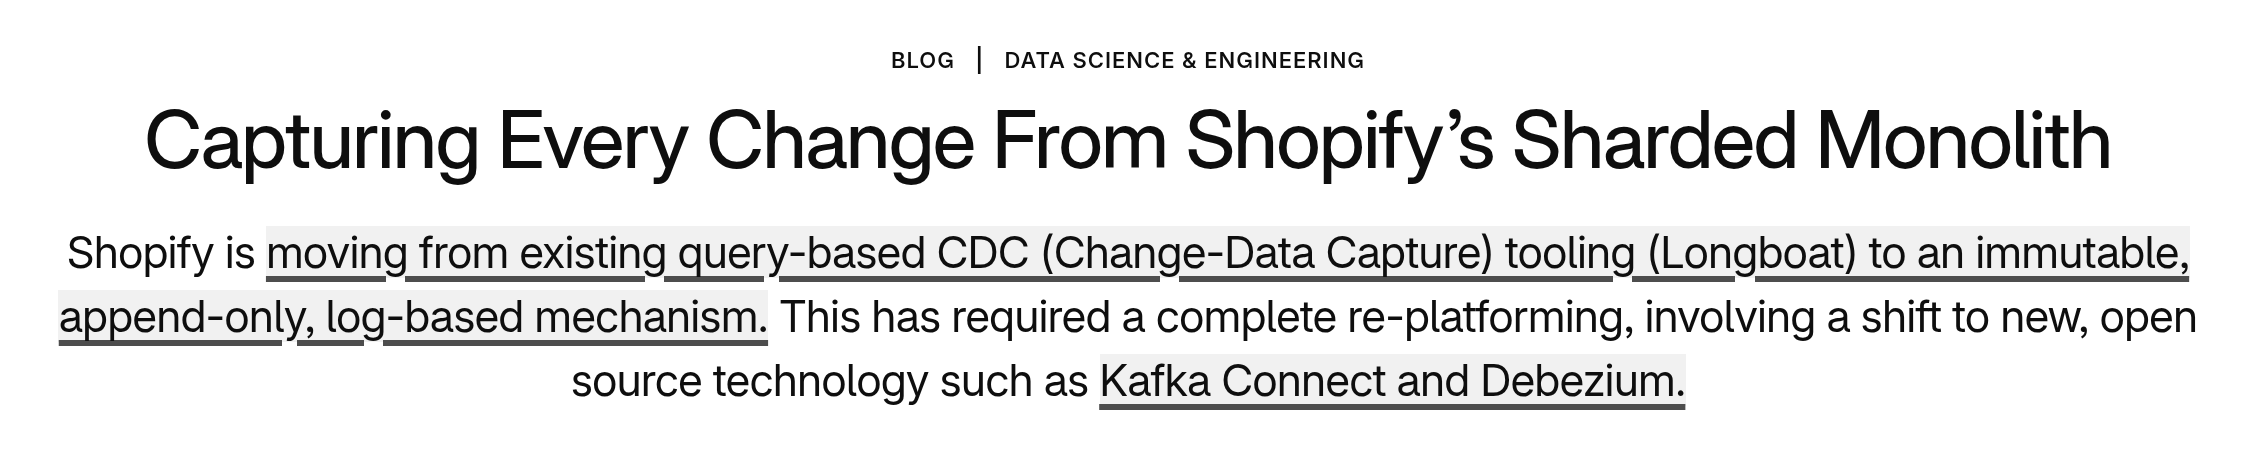
\includegraphics[width=\linewidth]{evidencias/grises/shopify-migracion.png}\par
}
\textbf{Figura 1.} Migración de Longboat a la captura de cambios mediante Kafka Connect y Debezium \cite{martin2021shopify}.

\vspace{8pt}
{\centering
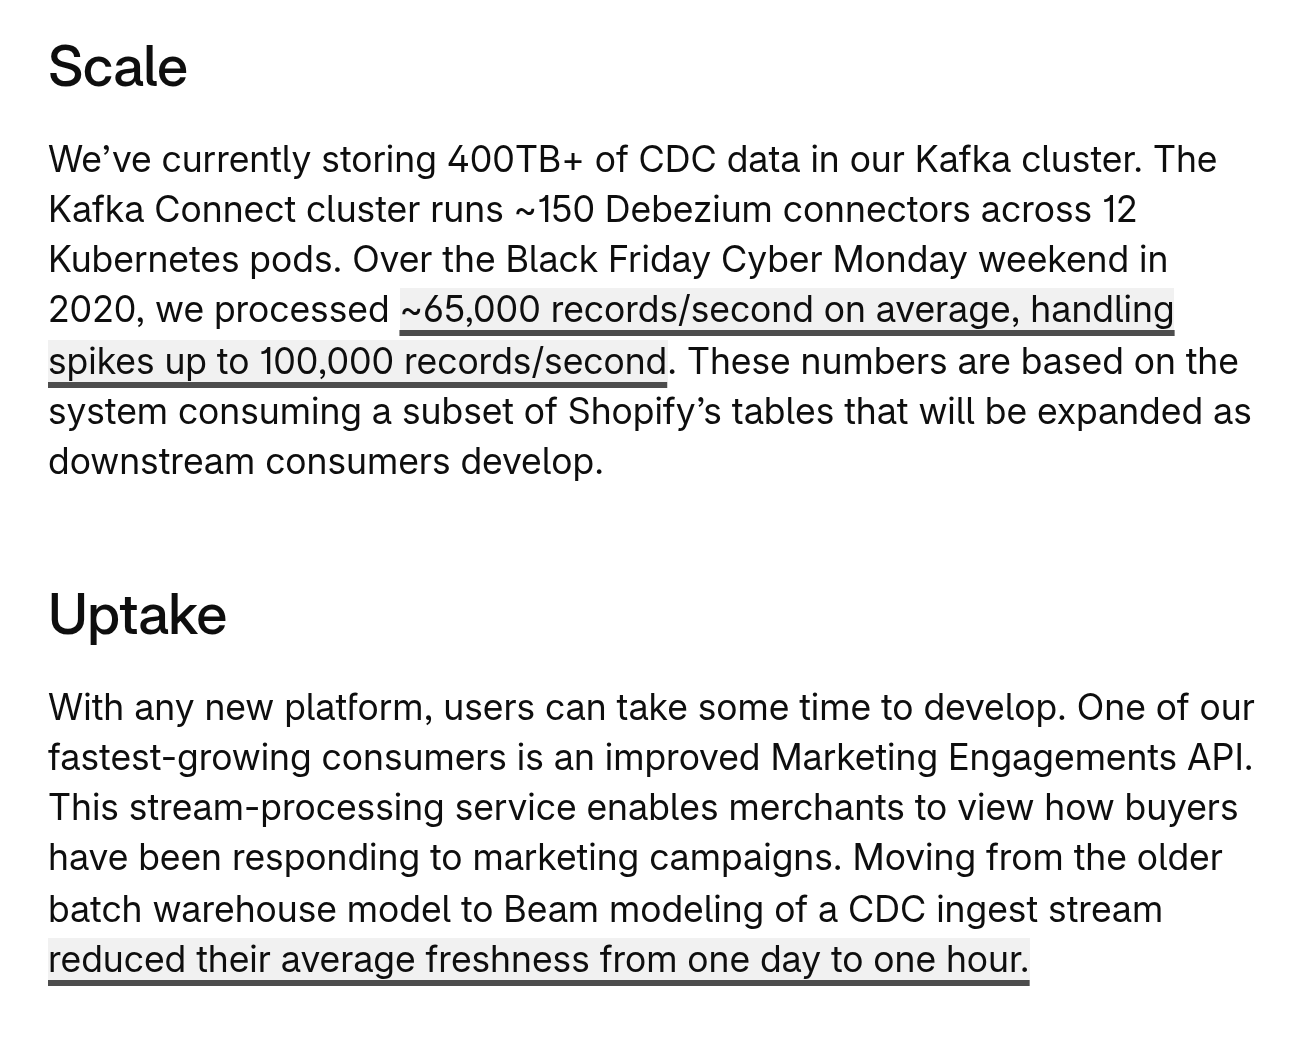
\includegraphics[width=.67\linewidth]{evidencias/grises/shopify-escala-y-beneficio.png}\par
}
\textbf{Figura 2.} Volumen de producción y desfase de los datos para la \textit{Marketing Engagements API} \cite{martin2021shopify}.

\vspace{8pt}
{\centering
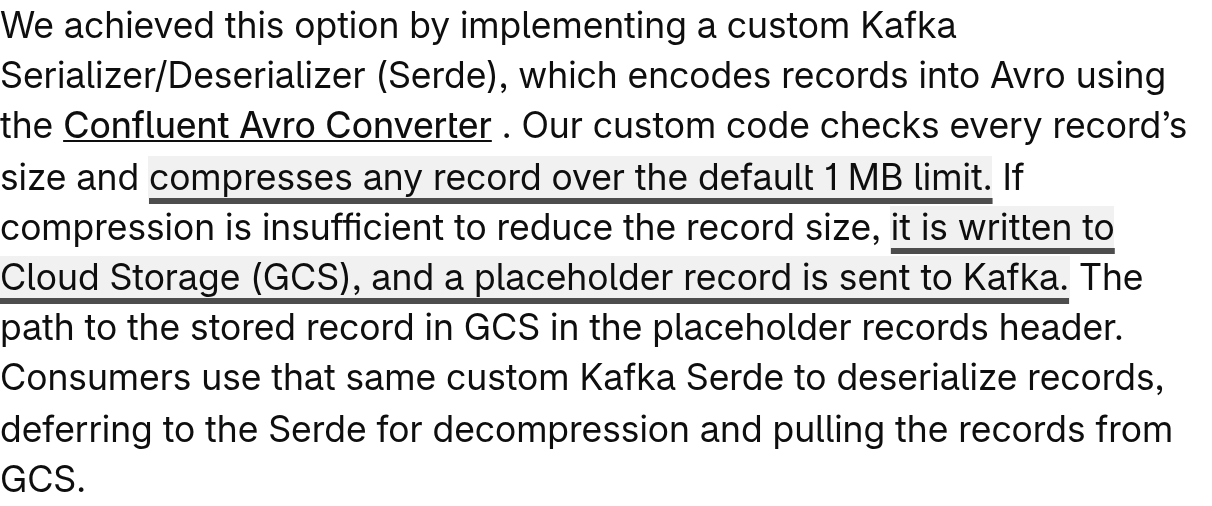
\includegraphics[width=.67\linewidth]{evidencias/grises/shopify-registros-grandes.png}\par
}
\textbf{Figura 3.} Compresión y almacenamiento externo de registros grandes \cite{martin2021shopify}.

\end{document}

